\documentclass{article}

\usepackage[utf8]{inputenc}

\usepackage{url}
\usepackage[hidelinks]{hyperref}

\usepackage{caption}

\usepackage{listings}

\usepackage{color}

% *** GRAPHICS RELATED PACKAGES ***
%\usepackage[pdftex]{graphicx}
\usepackage{graphicx}
%\usepackage[dvips]{graphicx}
% to place figures on a fixed position
\usepackage{float}

\usepackage[margin=1in]{geometry}

\title{OpenFlow \& Mininet – syllabus}
\author{}
\date{}


\begin{document}

\maketitle

\section{Introduction}

Today's networking devices vendors hide implementation details for trivial reasons, hence the researchers have a
serious problem testing new networking protocols, innovative ideas in real-world networks, under real-world conditions,
as there is no way to modify the details of the implementation. Naturally one can build test networks from consumer PCs
and running new switching or routing algorithms on these, but they operate on much lower speeds and has far less
processing power compared to carrier-grade switches, routers, which solve most tasks from hardware. This problem is
solved by the OpenFlow recommendation, which separates the internal operation of the switches and control logic,
enabling the option of programmable networks (SDN - Software Defined Networking). Thus, simple hardware-based basic
operations remain very fast and manufacturers do not have to disclose their details while the controller is separate
and programmable.

Before this lab, it is advisable to review the following lectures on Network Construction and Operation:

\section{OpenFlow recommendation}

OpenFlow is actually a system that provides a unified interface/protocol for modifying the behaviour of switches, so
they do not transmit packets according to the ``normal" mode of operation, but as determined by the programmer. This
description aims to briefly present the OpenFlow framework. For more details, please see the following documents:
\begin{itemize}
    \item Open Networking Foundation (OpenFlow Standardization Organization) \url{http://www.opennetworking.org/}
    \item Newer version of OpenFlow whitepaper: Software-Defined Networking: The New Norm for Networks
          \url{https://www.opennetworking.org/sdn-resources/sdn-library/whitepapers}
\end{itemize}

The project also aims to be interoperable with the existing networking infrastructure, meaning that traditional traffic
continues to processed by the networking devices while using OpenFlow to experiment with new packet forwarding
procedures. Accordingly, OpenFlow can be implemented in hardware switches (major manufacturers have already done this
in their products).OpenFlow is a relatively new technology that was released in 2008 at Stanford University. However,
as more and more companies started to be interested in this technology and started to use it more widely, the system's
shortcomings came to light that had been addressed by subsequent releases of the recommendation. As a result of the
contribution from major manufacturers and suppliers, the standardization activity grew beyond the academic environment
and a separate organization had been created (Open Networking Foundation). Currently Version 1.5 is the latest OpenFlow
recommendation, but in most cases the devices support version 1.0 only. There are, of course, some exceptions, and
there are now tools available that can work according to standard version 1.3.

It is important to note that currently version 1.0 is the most frequently used release however a significant change --
that affects the architecture of the hardware implementations -- was published between versions 1.0 and 1.1. Therefore
we will deal with these two versions in detail in this syllabus.

As from version 1.1, hardware variants are not that simple to be implemented (if you want to utilize the existing
elements and experiences), and nowadays software computing potential you can implement very powerful switch
implementations in plain software environments, significant improvements have also been made in this direction. Under a
software switch, we mean a solution that can run on a computer -- such as a desktop PC -- (in kernel or user space) and
can manage the network cards in the machine as separate switch ports.

Such software tools include the OpenFlow reference switch implemented at Stanford University, which operates in
user-space (which is, of course, less efficient); or Open vSwitch, which is a much more complex virtual switch in
kernel space that can be used not only for OpenFlow, but is used for example in an operating system virtualization
hosting software as a virtual network interface. (For Xen, this is the default virtual switch, but it is also supported
by VirtualBox.) The reference switches can also be ported to the OpenWRT environment, so it is possible to create
OpenFlow-capable switches from low-cost devices that run OpenWRT. Furthermore there are more expensive hardware devices
that are able to operate  according to the OpenFlow recommendation after the proper firmware upgrade. For example, HP
ProCurve 6600 that is also available in the lab inventory. For the sake of completeness, it should be noted that
OpenFlow was implemented on a NetFPGA card, where operation is implemented with re-programmable hardware devices
(FPGAs).

\subsection{OpenFlow system architecture}

OpenFlow's concept is based on the fact that most manufacturers' NPUs (Network Processing Unit) contains one or more
forwarding table - a.k.a. flow table - that controls the packet forwarding process. The OpenFlow standard separates the
devices into two categories as shown in Figure~\ref{fig:OpenFlow-arch}. The switch performs packet forwarding based on
its flow table, while the entries in the table are populated by an external controller. This allows switches to be
"dumb" devices, so there is no need for serious computing performance to run routing protocols etc. , as this is done
by a separate entity -- the controller.

An additional advantage is that the specific implementation can be proprietary as long as it is operating according to
the OpenFlow protocol and implementing the specification as the "programming" of the system is mainly performed via the
external controller, which is an open system.

It is important to mention that OpenFlow's packet transfer components are called switches, but these devices are
capable of much more compared to conventional L2 switches.
The L2 switches are capable of forwarding packets based on L2 headers. In some cases, this may be associated with
several extra functions (e.g. STP - Spanning Tree Protocol), but normally L3 headers are never inspected by a
traditional L2 switch.

In contrast, the OpenFlow switches are able to interpret the L2 and L3 header fields as described in more detail below.
This means that an OpenFlow switch can also have L3 routing implemented, i.e it can also function as an IP router.
Accordingly, the switch term refers to OpenFlow switches that are capable of packet forwarding both on L2 and L3 (even
L4) header fields.

\begin{figure}[!htb]
    \centering
    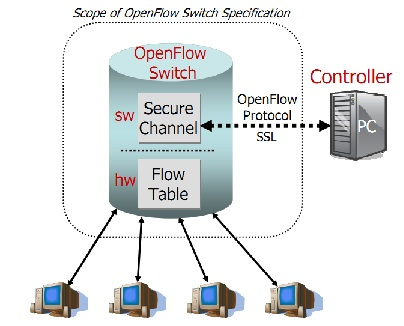
\includegraphics[width=0.9\textwidth]{figures/OpenFlow-architektura-2.jpg}
    \caption{OpenFlow architecture}
    \label{fig:OpenFlow-arch}
\end{figure}

The controller uses the OpenFlow protocol to communicate with the switches -- optionally via a secure channel. In
OpenFlow 1.1, it has appeared as a novelty in comparison to 1.0 that it has multiple flow tables, and there are not
just flow table, but also group tables which can be used for packet replication effectively - e.g IP multicast.
Multiple flow tables can be useful because one can group different types of process entries, for example, in the first
table ACL (Access Control List) information can be stored, while the second can be used for MPLS (MultiProtocol Label
Switching) entries and so on. The structure of the entries in the process tables is shown in
Table~\ref{tab:flow-entries}:

\begin{table}
    \centering
    \begin{tabular}[b] {| l | l  | l |}
        \hline
        Header fields & Counters & Actions \\
        \hline
    \end{tabular}
    \caption{Flow table entry structure}
    \label{tab:flow-entries}
\end{table}

The header fields are those parts of the packet headers that are used by the switch to make the forwarding decision by
finding a matching flow entry in the flow table. The fields that are used as the flow key for the lookup are show in
Table~\ref{tab:flow-key}

\begin{table}
    \centering
    \begin{tabular}[b] {| l |}
        \hline
        Ingress port             \\ \hline
        Meta-data                \\ \hline
        Source MAC address       \\ \hline
        Dest. MAC address        \\ \hline
        Ether type               \\ \hline
        VLAN id                  \\ \hline
        VLAN priority            \\ \hline
        MPLS label               \\ \hline
        MPLS class of service    \\ \hline
        IPv4 source address      \\ \hline
        IPv4 destination address \\ \hline
        IP Protocol              \\ \hline
        IPv4 ToS                 \\ \hline
        Source TCP/UDP port      \\ \hline
        destination TCP/UDP port \\
        \hline
    \end{tabular}
    \caption{Flow key structure}
    \label{tab:flow-key}
\end{table}

All but the meta-data fields are well specified. Meta-data is used by OpenFlow to exchange information between tables,
as the packet can go through several tables during processing, searching for a matching entry, but a match in one table
may affect the search in a subsequent table. The meta-data field is suitable for transmitting these kind of information
and it is stored in 64 bits.

Packages arriving to the OpenFlow switch go into a pipeline where forwarding decision will be made. This is illustrated
on Figure~\ref{fig:OpenFlow-pipeline}.

\begin{figure}[!htb]
    \centering
    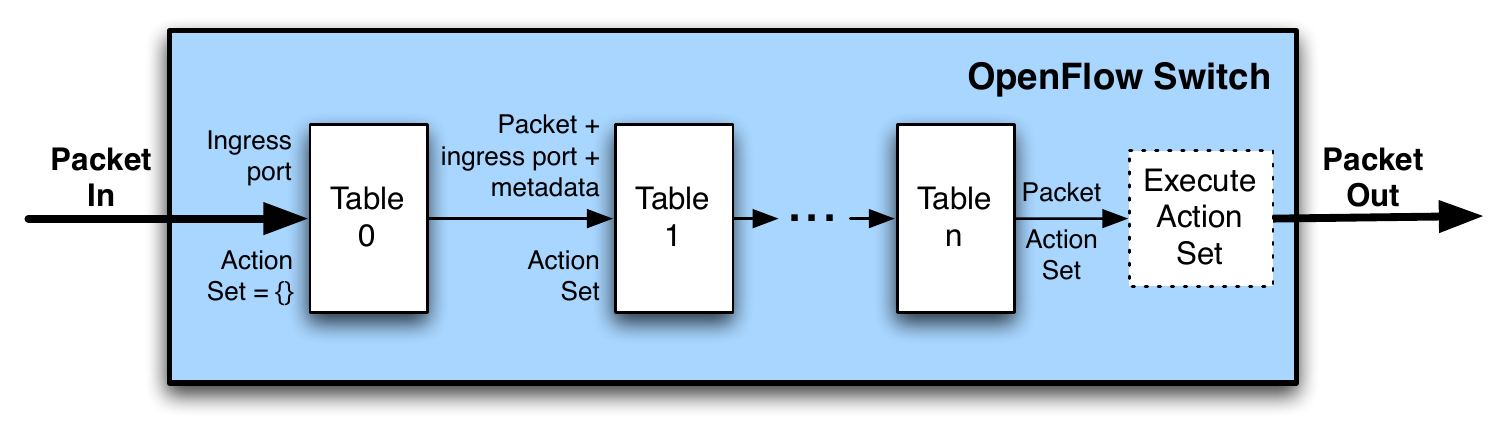
\includegraphics[width=0.9\textwidth]{figures/table-pipeline.png}
    \caption{Packet processing pipeline}
    \label{fig:OpenFlow-pipeline}
\end{figure}

The incoming packets go through the tables one after another until a match is found in any of the entries. If the
package matches an entry, the counters of that entry are updated and the related instructions/actions are executed.
Also as shown in Figure~\ref{fig:OpenFlow-pipeline}, between the pipeline stages the packet, the associated meta-data
and the action set to be performed are being forwarded conceptionally.

When the packet reaches the end of the last flow table or there is an instruction in the matching entry to execute the
actions, the actions in the action set will be executed. After that, the packet either leaves the switch on the
corresponding port (s) or it is discarded. Figure~\ref{fig:OpenFlow-matching-process} augments this process with the
possibility of a jump between tables and shows what happens when a matching entry is not found in a table.
The \emph{`Drop'} terminal on Figure~\ref{fig:OpenFlow-matching-process} -- based on the table configuration -- can be
either :

\begin{itemize}
    \item send to controller
    \item drop
    \item continue with next table
\end{itemize}

\begin{figure}[!htb]
    \centering
    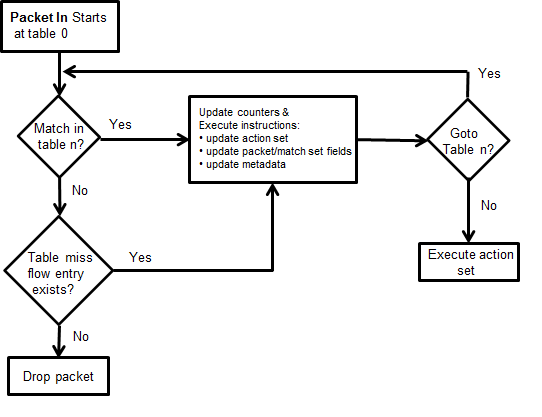
\includegraphics[width=0.9\textwidth]{figures/openflow-processing-flowchart.png}
    \caption{Flow entry matching process}
    \label{fig:OpenFlow-matching-process}
\end{figure}

Figure~\ref{fig:OpenFlow-matching-process} also emphasizes the role of the controller: if the switch doesn't find a
matching entry during the flow table lookup it potentially embeds the packet in an OpenFlow packet and it sends that to
the OpenFlow controller using the OpenFlow protocol. The controller can then act accordingly -- it can simply ignore
the event, or alternatively it can install new	or modify existing flow entries, or it can inject control packets into
the network.

The flow entries can contain the following instructions:
\begin{itemize}
    \item \emph{`Execute action set'} : execute some immediate action(s) without affecting the action set of the
          packet
    \item \emph{`Delete action set'} : this will empty the action set
    \item \emph{`Write meta-data'} : write some appropriately masked meta-data into the packet associated meta-data
          register
    \item \emph{`Goto Table'} : specifies that in which subsequent table should the switch continue the lookup
          procedure. The table ID must be greater than the current table id.
\end{itemize}

The action set can contain the following actions:
\begin{itemize}
    \item Send out packet on a specific port. The port can be physical or logical like for example the
          \emph{Controller port} or \emph{All} which can be used to send out packets on all ports
    \item Drop packet
    \item Send to group table
    \item Modify various packet header fields
\end{itemize}

\subsubsection{OpenFlow 1.0 simplifications, differences}

In OpenFlow 1.0 specification there is only one flow table instance, so there is no pipeline, and there are actions
directly instead of instructions because as there is no need to collect the actions in each table. In reality there are
more than one table present in the v1.0 implementations. A typical software implementation has two of them -- the first
one is a hash table, in which the so-called exact match entries are stored. These entries have all the header fields
data populated which are specified in the OpenFlow specification used for matching. The second is used for storing the
so-called \emph{`wild-card'} entries. Typical implementation is that the wild-card entry is accompanied with a bit mask
that is applied to the packet data used in the matching process. As a result some fields can be excluded from the
packet forwarding decision.  For example, for HP hardware devices used in this lab, also have a third flow table with
hardware acceleration. (But these tables are not operating in a pipeline!)

\subsection{The OpenFlow channel}

The OpenFlow enabled switches connect to the controller via this interface. The channel can be established over TLS
(Transport Layer Security) encrypted or unencrypted TCP connection. Communication over the OpenFlow channel is done
through the OpenFlow protocol. The protocol distinguishes three message types, these are the router-switch,
asynchronous, and symmetric messages.

Controller-switch messages are initiated by the controller and the switch may not always respond to them. For example,
configuring the switch or querying its capabilities falls into this category but statistics queries or flow table
modifications are also belong to this category.

In contrast, asynchronous messages are sent by the switch to the controller in an unsolicited manner. These messages
for example can indicate changes in  operational state change of switch ports (up / down), other errors, removal of
flow entries due to time-out, or if there is no matching entry for a packet that is transmitted to the controller in
this way.

Symmetric messages can be initiated by either party unsolicited but the originator expects a reply for these types of
messages. This includes the \emph{Hello} message used for channel establishment, and the \emph{Echo} message that is
used for keep-alive mechanism and measuring the bandwidth of the channel.

\section{Controllers - NOX controller}

The most important element of an OpenFlow-based network is the controller that controls the switches. It is essential
that the controller and the controller-switch connection are functioning properly for the normal operation of the
network. There are several suggestions for implementing redundancy, such as a distributed controller or redundant
connections.
However, if the controller-switch is still down, two operating modes are possible according to the specification. One
is \emph{``fail secure mode"}. In this mode the switch will continue to operate using the existing entries (but they
still removed if a time-out is configured for them) and it drops the packets destined to the controller -- a.k.a
\emph{``headless mode"}. This mode of operation provides resiliency in case of short interruption of the
switch-controller channel.

Another mode is the "fail standalone mode". In this mode, the switch will return to traditional mode, i.e. without
using OpenFlow, it will operate as a conventional Ethernet switch. This mode can also be operational in case of a
longer controller failure, but the network may not work according to expectations. The preferred mode of operation in
case of controller outage can be configured freely in the switch.

Today, a number of control platforms are available to use, where network applications can be developed using different
software environments and programming languages/paradigms. One of the earliest, oldest controllers is called NOX. The
NOX Controller was basically designed for the most efficient operation in mind, currently this platform -- implemented
in C++ -- provides the best performance in term of the number of streams served under a period of time (for a
conventional desktop PCs -- which, of course, can mean anything -- that means more than 10,000 new streams per second).
The trade-off for efficiency and relatively good scalability is the not so convenient programming environment  using
C++ language. The goal of the creators of NOX is to create a network operating system (see NOX: Towards an Operating
System for Networks). In this context Networking Operating System means that the software is not intended to manage the
network, but it provides a well-defined programming interface for the network itself that makes it is easier to
implement the centralized control of the networking equipments from different vendors and to write portable and
re-usable control programs that implement some networking functionality. They have created an analogy with traditional
operating systems, as they are hiding the details of the underlying hardware and have well-defined programming
interfaces that allows the developers to write portable, higher-level programs. NOX can be programmed in python as
well, but there is a pure python-based controller is available called POX. That is implemented entirely in python,
while in the classical version the core is implemented in C++ and python bindings are provided to be able use it from
python.

POX provides a much clearer, simpler programming environment, especially useful for rapid prototyping and educational
purposes. One disadvantage (perhaps) is that it currently only supports version 1.0 of OpenFlow. Several other
controllers are available, such as Floodlight (Java based), OpenDaylight (also a Java based but enterprise grade), Ryu
(python based), Trema (ruby or C language programmable) or higher abstraction such as Frenetic (declaratively
programmable), ONOS (a network operating system).

The NOX controller is also available for OpenFlow versions 1.1, 1.2, 1.3 and 1.4 which is used for demonstration in the
following examples. NOX has a modular architecture and it can be extended with custom made applications where existing
functionalities (e.g. discovery modules) can be re-used as well. The applications can be implemented using C ++ or
Python.

NOX implements the central control using the OpenFlow protocol, as it's shown on Figure~\ref{fig:NOX-network}.
The system itself runs on one or more central servers. The OpenFlow switches connect to the servers through which the
network can be controlled. The server also runs additional applications beside the controller (typically one more) that
uses the NOX API to manage the network. The network view -- as seen by NOX -- is stored in a database called
\emph{`Network View'}. The view is created dynamically by querying information from each OpenFlow switch.

\begin{figure}[!htb]
    \centering
    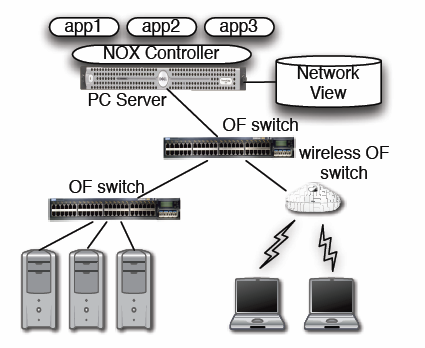
\includegraphics[width=0.9\textwidth]{figures/NOX_Networks.png}
    \caption{The components of a NOX based network}
    \label{fig:NOX-network}
\end{figure}

\subsection{Demonstration of operation on a simple topology}

In this section a simple OpenFlow based topology is presented on which the operating principles can be demonstrated in
practice. The topology is illustrated by Figure~\ref{fig:NOX-sample-topo} (and it is actually emulated using the
Mininet framework presented in Section~\ref{sec:Mininet})

\begin{figure}[!htb]
    \centering
    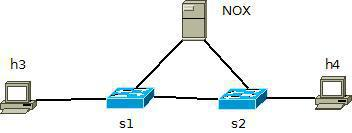
\includegraphics[width=0.9\textwidth]{figures/sample_topology.jpg}
    \caption{Sample topology}
    \label{fig:NOX-sample-topo}
\end{figure}

The topology consists of two switches and two host attached to each of it -- the identifiers used can be read from
Figure~\ref{fig:NOX-sample-topo}.
The switches are connected to a NOX based controller on which a typical MAC address learning application is running.
Querying the flow entries from the switches makes it clear that all flow tables are empty after start-up (see
Figure~\ref{fig:NOX-empty-flowtable}) similarly to a conventional L2 switch with an empty MAC table that is populated
dynamically as source MAC addresses are observed of incoming packets. Despite that the switches have been discovered by
the controller furthermore the connected devices are also visible (network view, the controller is topology aware)

\begin{figure}[!htb]
    \centering
    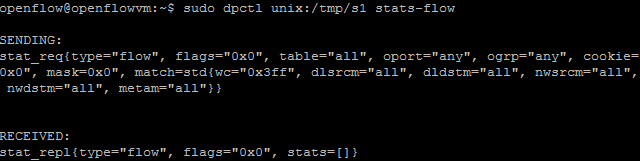
\includegraphics[width=0.9\textwidth]{figures/empty_flowtable.png}
    \caption{Empty flow table after start-up}
    \label{fig:NOX-empty-flowtable}
\end{figure}

After initialization a ping is executed from host \emph{h3} to \emph{h4} that results in a bidirectional flow
establishment in a way that corresponding flow entries are populated into the flow table's of the switches. The flow
entries after the ping are shown by Figure~\ref{fig:NOX-populated-flowtable}.

\begin{figure}[!htb]
    \centering
    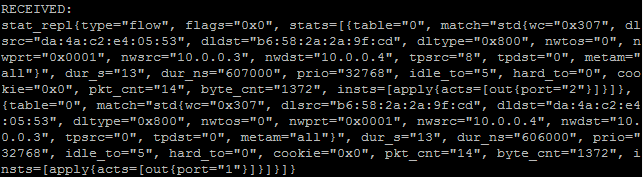
\includegraphics[width=0.9\textwidth]{figures/populated_flowtable.png}
    \caption{Populated flow table}
    \label{fig:NOX-populated-flowtable}
\end{figure}

As a result of inspecting the ping messages timing it is clear that the forwarding time of the first packet takes
considerably longer time (2.33 ms) compared to the subsequent packets (0.06-0.2 ms) because the flow entries are
populated as the controller reacts to the OpenFlow messages triggered by the first packet events as illustrated by
Figure~\ref{fig:NOX-ping}

\begin{figure}[!htb]
    \centering
    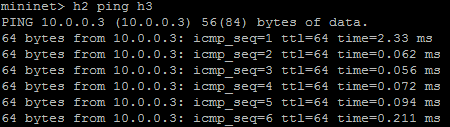
\includegraphics[width=0.9\textwidth]{figures/ping_example.png}
    \caption{Ping messages and their timings}
    \label{fig:NOX-ping}
\end{figure}

The flow tables provisioning is done by sending the corresponding flow mod messages.
Figure~\ref{fig:NOX-populated-flowtable} shows that two entries have been added in table 0. -- as expected -- , that
represent bi-directional forwarding with the corresponding dl\_src and dl\_dst MAC addresses set furthermore the IP
addresses have been provisioned also. These entries do not contain wild-cards so the controller was able to fill our
each mandatory field in the flow key. In contrast to this a conventional L2 switch only forwards based on the
destination MAC address and floods the packet if the destination address is unknown.

Such wild-carded entries can be created in the OpenFlow framework so that the masked out parts of the flow key do not
participate in the matching process. It can be also observed that the entries have a 5 seconds inactivity time-out --
after which they are removed -- plus the Instructions to be carried out are also there.

The OpenFlow control messages can be monitored using Wireshark packet capture software over the control interface.
Currently only OpenFlow v1.0 has an adequate protocol dissector plug-in.

\subsection{OpenFlow v1.0 differences and simplifications}

In OpenFlow version 1.0 the structure of the flow entries are much simpler and dumping the flow table is done slightly
differently. Figure~\ref{fig:NOX-table-dump-v1.0} shows a table dump from a switch running on localhost using the
\emph{dpctl} command.

\begin{figure}[!htb]
    \centering
    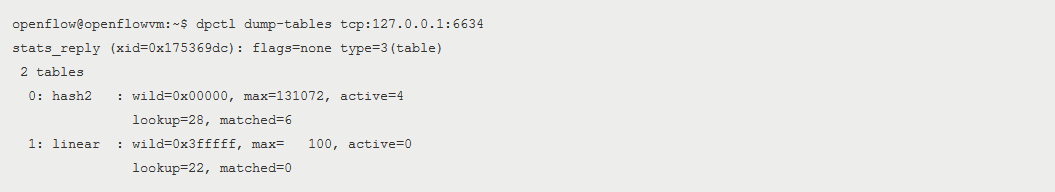
\includegraphics[width=0.9\textwidth]{figures/table_dump.png}
    \caption{OpenFlow v1.0 table dump}
    \label{fig:NOX-table-dump-v1.0}
\end{figure}

From the result returned by the switch it is visible that currently there are 4 active entries and all of these are
situated in the \emph{hash} table. If one would like to inspect concrete flow entries the \emph{dpctl} utility can be
used with proper arguments as shown on Figure~\ref{fig:NOX-entries-dump-v1.0}

\begin{figure}[!htb]
    \centering
    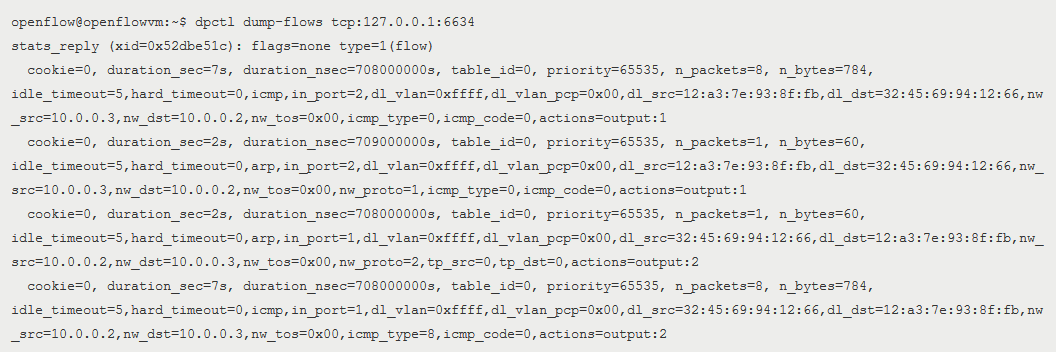
\includegraphics[width=0.9\textwidth]{figures/entry_dump.png}
    \caption{OpenFlow v1.0 entries dump}
    \label{fig:NOX-entries-dump-v1.0}
\end{figure}

Out of the 4 entries 2 are there for ICMP packets while the remaining 2 are for ARP packets. Since the hash table uses
exact matching all fields of the flow key entries are fully populated. For example decoding the 1st entry says that if
an ICMP packet arrives on port no. 2 (in\_port=2) that has source IP address as 10.0.0.3 and destination IP address as
10.0.0.2 etc. then the matching packet has to be forwarded over port 1 (actions=output:1). Several other parameters can
be tweaked like e.g priority of the entry, time-out, etc. Further information can be found related to this on the man
page of the \emph{dpctl} command.

\section{Mininet}\label{sec:Mininet}

Mininet is an extremely useful network simulator software tool which is capable of emulating OpenFlow networks
consisting from hundreds of OpenFlow switches using on a single host computer.

It was designed for emulating large-scale network with minimal resource utilization. It is possible to emulate networks
with more than 100 hosts on a single laptop. This is possible via using OS level virtualization facilities, host are
realized as standalone shell processes and network namespaces. The main goal of this tool is to make it possible to
experiment with new network architectures, addressing schemes, etc. using only consumer class PCs. The following design
principles were established by the authors of Mininet:
\begin{itemize}
    \item Flexibility: testing new functionality in software running on a well-known OS
    \item Install-ability: The potential of installing a functionally complete model onto real hardware
    \item Interactivity: The network management and operation must be real-time just like in a real world network
    \item Scalability: Must scale in a way that hundreds of devices can be emulated by using a single laptop
    \item Realistic: The operation itself should be as close as it can be compared to the real world
    \item Sharing: the sharing of prototypes should be done with ease amongst the developers working on the same
          projects
\end{itemize}

Before Mininet came there were expensive special purpose devices for network emulation or alternatively software
simulators (e.g ns-2) that were not realistic enough. Mininet addresses these issues by having a Python implementation
running on Linux OS. The host and node emulation is performed using shell processing, virtual Ethernet pairs and
network namespaces. For testing new topologies and network architectures and algorithms it uses the OpenFlow standard.
The internal implementation of Mininet is illustrated by Figure~\ref{fig:Mininet-Impl}

\begin{figure}[!htb]
    \centering
    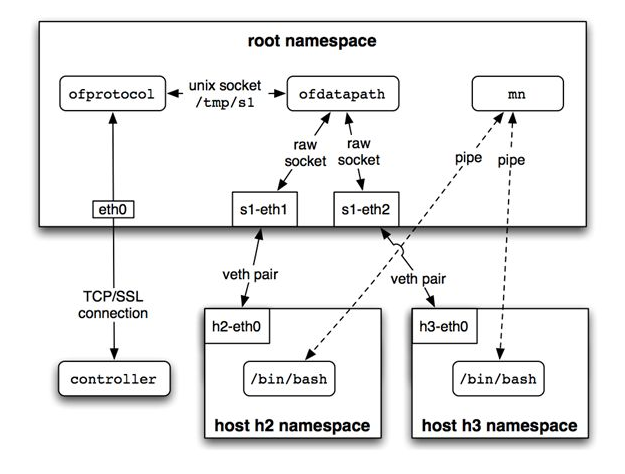
\includegraphics[width=0.9\textwidth]{figures/mininet_impl.png}
    \caption{Mininet implementation details}
    \label{fig:Mininet-Impl}
\end{figure}

Mininet instead of using virtual machines for each individual host uses a more light-weight solution: it launches
simple shell processes for them where each host has a corresponding shell process associated with it that can execute
arbitrary programs. Each process is launched in a separate network namespace so that is has its own network interface,
routing table etc. From networking perspective it behaves as a standalone entity. The virtual interfaces are
interconnected with the corresponding switch port running in the root namespace using virtual connections. The host
processes can communicate with Mininet using the OS pipe facilities so that each host can be controlled respectively.
The switches can be connected to an external controller that can run either on a remote machine or on the local host.

When starting Mininet one can specify to which software switch implementation should it run, how should it connect to
the controller, what is the network topology it should emulate and also that which internal test suites should it
execute.
There are multiple options present for selecting the the controller. Either a reference controller or the previously
mentioned NOX controller can be used, which could be launched either by Mininet or manually. In the latter case only
the controller's IP address and port has to be specified. For the switch implementation there are also two
possibilities. One of them is the OpenVSwitch that supports OpenFlow v1.0 or alternatively the reference switch
implementation can be used. The internal test suite consists two test cases: the ping test, that verifies the
availability of the hosts, and the iperf test, which measures the transmission bandwidth between two hosts.

\begin{figure}[H]%[!htb]
    \centering
    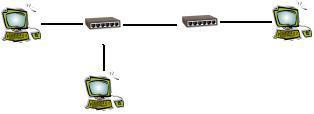
\includegraphics[width=0.9\textwidth]{figures/mininet-topology.jpg}
    \caption{A sample topology in Mininet}
    \label{fig:Mininet-sample-topo}
\end{figure}

There are multiple options for specifying the network topology as well. A couple of simple topologies have been
embedded into Mininet itself --like linear or tree topology -- where only some parameters has to be specified.
There is also an option for describing custom topologies manually using Python code. For example topology on
Figure~\ref{fig:Mininet-sample-topo} is described with the code of Figure~\ref{fig:Mininet-sample-topo-code}.

\begin{figure}[H]%[!htb]
    \centering
    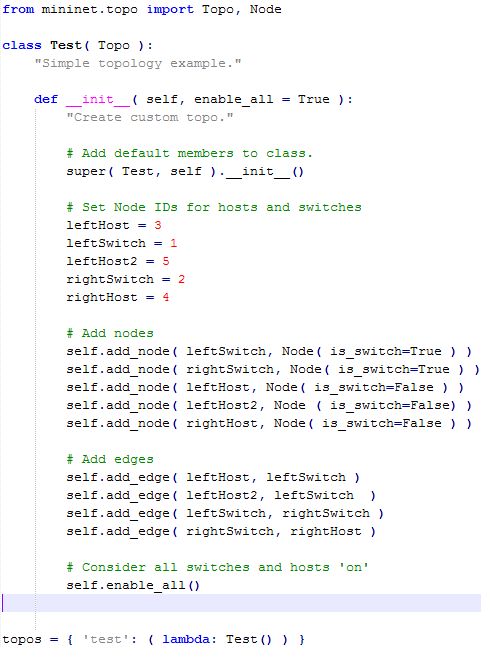
\includegraphics[width=0.9\textwidth]{figures/mininet-code.png}
    \caption{Sample Mininet topology's Python description}
    \label{fig:Mininet-sample-topo-code}
\end{figure}

Starting from newer Mininet versions (v2.0) there is a new method for describing topologies as shown in
Listing~\ref{lst:Mininet-2.0-example}

\lstinputlisting[language=Python,showstringspaces=false,frame=single,breaklines,caption={Mininet 2.0 newer topology
            specification scheme},label=lst:Mininet-2.0-example]{resources/mininet-2.0-sample.py}

Listing~\ref{lst:Mininet-2.0-example} shows that the topology can be described with relative ease. First it sets up the
identifiers of the devices then -- by calling self explanatory functions -- it creates the virtual devices and the
interconnections between them. After these steps it fires up the devices. Starting from there the topology can be
launched from Mininet by specifying the appropriate switches on the command line as shown by
Listing~\ref{lst:Mininet-startup}

\begin{lstlisting}[language=bash,frame=single,breaklines,caption={Mininet startup command},label=Mininet-startup]
sudo -E mn  --switch=user --controller=remote --ip=127.0.0.1 --port=6633 --custom /home/openflow/mininet/custom/topo-test2.py --topo test
\end{lstlisting}

As a result of the command execution of Listing~\ref{lst:Mininet-startup} Mininet starts the reference switch
implementation which will connect to a controller listening on localhost:6633 and it also loads the user defined
topology as given. After startup  commands can be executed on arbitrary selected hosts by entering the host identifier
and the command to execute (e.g. h3 ping h4). Furthermore if a \emph{ssh} daemon is running on the virtual hosts
connecting to them using ssh is also possible even with using X window forwarding.

One of its greatest advantages of Mininet is that solutions developed using Mininet can be easily ported to real
hardware devices. This results in quick and effective development cycles without the availability of real networking
equipment at hand. The controller application running in Mininet is capable of communicating with both virtual and
non-virtual devices as well as long as they conform with the OpenFlow specification.

\section{Further Reading}

On mininet:
\begin{itemize}
    \item \href{https://qosip.tmit.bme.hu/foswiki/pub/Meres/OpenFlowMScMeresiSegedlet/a19-lantz.pdf}{A Network in a
              Laptop: Rapid Prototyping for Software-Defined Networks}
    \item
          \href{https://qosip.tmit.bme.hu/foswiki/pub/Meres/OpenFlowMScMeresiSegedlet/mininet-hotnets2010-final.pdf}{Presentation
              of conference proceedings on Mininet}
    \item	Mininet page: \url{http://mininet.org/}
    \item	Mininet wiki: \url{https://github.com/mininet/mininet/wiki}
    \item	Mininet introduction: \url{https://github.com/mininet/mininet/wiki/  Introduction-to-Mininet}
    \item	Mininet Python API: \url{http://mininet.org/api/hierarchy.html}
\end{itemize}

OpenFlow specifications:
\begin{itemize}
    \item
          \href{https://qosip.tmit.bme.hu/foswiki/pub/Meres/OpenFlowMScMeresiSegedlet/openflow-spec-v1.0.0.pdf}{v1.0}
    \item
          \href{https://qosip.tmit.bme.hu/foswiki/pub/Meres/OpenFlowMScMeresiSegedlet/openflow-spec-v1.1.0.pdf}{v1.1}
    \item
          \href{https://qosip.tmit.bme.hu/foswiki/pub/Meres/OpenFlowMScMeresiSegedlet/openflow-switch-v1.3.4.pdf}{v1.3.4}
    \item
          \href{https://qosip.tmit.bme.hu/foswiki/pub/Meres/OpenFlowMScMeresiSegedlet/openflow-switch-v1.4.1.pdf}{v1.4.1}
    \item
          \href{https://qosip.tmit.bme.hu/foswiki/pub/Meres/OpenFlowMScMeresiSegedlet/openflow-switch-v1.5.1.pdf}{v1.5.1}

\end{itemize}

\end{document}